\section{Answer to Question \ref{q:why}: The cause of clusterization}\label{section:why}


%% In the inverse problem of the heat equation, \ev_3, \ev_4,\dots$
%% implies we seek measurement locations for which $\lambda_1\ev_1,
%% \lambda_2\ev_2$ are large, while $\lambda_3\ev_3,
%% \lambda_3\ev_3,\dots$ are small. It turns out that there are two
%% locations that give the best trade-off, and measurements are taken in
%% those two locations. Once we have more than two measurements at our
%% disposal, measurement locations becomde clustered, by the pigeonhole
%% principle, see Fig.~\ref{fig:eigenvectors}.

%% The way a D-optimal design tries to ignore all eigenvectors
%% corresponding to $j > 2$. Since $\lambda_j$ decay to zero, a D-optimal
%% design should only try to avoid eigenvectors for which $\lambda_j$ is
%% not already small --- e.g.~eigenvectors $j=3,4$. It is possible that
%% the geometry of the domain $\Omega$ and the structure of the
%% eigenvectors leave only a few locations in $\Omega$ where the
%% amplitude of eigenvectors $j=1,2$ is high while the amplitude of
%% eigenvectors $j=3,4$ is low. In such case, clusterization will occur
%% whenever the number of measurements $m$ is large enough, by the
%% pigeonhole principle. This scenario is illustrated for the inverse
%% problem of the 1D heat equation in Fig.~\ref{fig:eigenvectors}.

\begin{figure}\label{fig:eigenvectors}
    \centering
    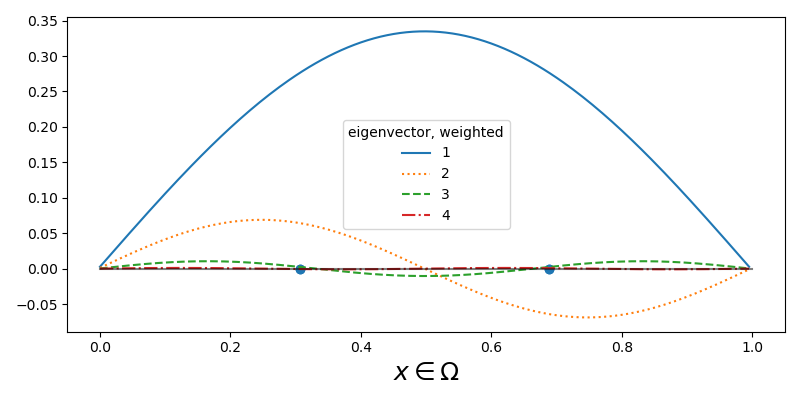
\includegraphics[width=\textwidth]{eigenvectors_dst_scaled.png}
    \caption{D-optimal measurement locations ($m=4$ measurements) and
      weighted eigenvectors for finding the initial condition of
      the 1D heat equation. Measurement locations and weighted
      eigenvectors are plotted over the computational domain $\Omega =
      [0, 1]$ (x-axis). Measurement clusterization occurs
      approximately at $0.31$ and $0.69$. These two locations are a
      compromise between zeros of eigenvectors a D-optimal design aims
      to ignore (third and up) and staying far from zeros of the
      eigenvectors a D-optimal design aims to measure (first and
      second). Allocating $m=4$ measurements into two locations
      results in clusterization, according to the pigeonhole
      principle.}
  \label{fig:why}
\end{figure}




%% According to Theorem \ref{thm:char}, D-optimal designs aim to capture
%% a small subset of eigenvectors of the prior covariance, specifically
%% the $k$ eigenvectors with the highest prior variance. Our model
%% naturally achieves this objective by not measuring eigenvectors $k+1$
%% and above, as proven in Theorem \ref{thm:char}. Translating this
%% understanding to spatial problems, we anticipate that a D-optimal
%% design would favor measurement locations where eigenvectors $k+1$ and
%% above are either close to zero in value or possess small eigenvalues
%% in the prior spectrum, for some $k > 0$. To illustrate this
%% preference, Fig.~\ref{fig:why} depicts the scenario using the 1D
%% heat equation with homogeneous Dirichlet boundary conditions (details
%% in the supplementary material). The plot showcases four eigenvectors,
%% scaled according to their prior standard deviations. Since
%% eigenvectors beyond the fourth have insignificant prior eigenvalues,
%% we exclude them from consideration. Notably, we observe that
%% measurements are clustered near the zeros of the third and fourth
%% eigenvectors, so we conclude that $k=2$. Clusterization arises because
%% there are only two locations where the third and fourth eigenvectors
%% approach zero, while the first and second eigenvectors exhibit
%% significantly non-zero values. Consequently, when we allocate four
%% measurements to these two locations, they naturally cluster together,
%% aligning with the pigeonhole principle.
